\documentclass[a4paper]{article}

%% Language and font encodings
\usepackage[english]{babel}
\usepackage[utf8x]{inputenc}
\usepackage[T1]{fontenc}

%% Sets page size and margins
\usepackage[a4paper,top=3cm,bottom=2cm,left=2.7cm,right=2.7cm,marginparwidth=1.75cm]{geometry}

%% Useful packages
\usepackage{amsmath}
\usepackage{amsfonts}
\usepackage{bm}
\usepackage{graphicx}
\usepackage[colorinlistoftodos]{todonotes}
\usepackage[colorlinks=true, all colors=blue]{hyperref} %referenze linkate
\usepackage{booktabs}
\usepackage{siunitx}  %notaz. espon. con \num{} e unità di misura in SI con \si{}
\usepackage{xcolor}
\usepackage{colortbl}
\usepackage{bm}
\usepackage{caption} 
\usepackage{indentfirst}
\usepackage{physics} 
\usepackage{rotating}
\usepackage{tabularx}
\usepackage{url}
\usepackage{pst-plot}
\usepackage{comment} %per usare l'ambiente {comment}
\usepackage{float} 
\usepackage{subfig}
\usepackage[americanvoltages]{circuitikz} %per disegnare circuiti
\usepackage{tikz}
\usepackage{mathtools} %per allineare su più linee in ambiente {align} o {align*}
\usepackage{cancel}
\usepackage{listings}
\renewcommand{\CancelColor}{\color{lightgray}}
%\setlength{\parindent}{0cm}


%%%%%%%%%% HEADERS AND FOOTERS %%%%%%%%%%%%
\newcommand{\theexercise}{Ex. 4}
\newcommand{\thedate}{November 2, 2020}
\usepackage{fancyhdr}

\pagestyle{fancy}
\fancyhf{}
\lhead{Giorgio Palermo}
\rhead{\thedate}
\lfoot{Quantum Information 20/21}
\cfoot{\theexercise}
\rfoot{Page \thepage}

%%%%%%%%%% CODE LISTING %%%%%%%%%%%
%New colors 
\definecolor{codegreen}{HTML}{92c42a}
\definecolor{codegray}{rgb}{0.5,0.5,0.5}
\definecolor{codepurple}{HTML}{f92472}
\definecolor{codeblue}{HTML}{67d8ef}
\definecolor{codeyellow}{HTML}{e68f29}%{e4ab24}
\definecolor{codemagenta}{HTML}{f92472}
\definecolor{backcolour}{rgb}{0.95,0.95,0.92}


%Code listing style named "mystyle"
\lstdefinestyle{mystyle}{
  language={[03]Fortran},
  backgroundcolor=\color{backcolour},   commentstyle=\color{codegray},
  keywordstyle=\color{codemagenta},
  numberstyle=\tiny\color{codegray},
  stringstyle=\color{codeyellow},
  basicstyle=\ttfamily\footnotesize,
  breakatwhitespace=false,         
  breaklines=true,                 
  captionpos=b,                    
  keepspaces=true,                 
  numbers=left,                    
  numbersep=5pt,                  
  showspaces=false,                
  showstringspaces=false,
  showtabs=false,                  
  tabsize=2
}
%"mystyle" code listing set
\lstset{style=mystyle}


\graphicspath{{Figure/}}
\captionsetup{format=hang,labelfont={sf,bf},font=small}
\captionsetup{tableposition=top,figureposition=bottom,font=small}
\captionsetup[table]{skip=8pt}







\begin{document}
\hypersetup{linkcolor = black}
\hypersetup{linkcolor = blue}
\thispagestyle{plain}
\begin{center}
    \textbf{MASTER'S DEGREE IN PHYSICS}
    
    Academic Year 2020-2021
    
    \medskip
    \textbf{QUANTUM INFORMATION}
\end{center}

\vspace{0.0cm}
Student: Giorgio Palermo

Student ID: 1238258

Date: \thedate
\begin{center}
\textbf{EXERCISE 4}
\medskip
\end{center}
\noindent
\textit{In this report I will describe the details on how I tested the performance of my machine relative to matrix multiplication using Fortran subroutines and Python scripts; I will briefly evaluate trend of the data I obtained for matrices of sizes spanning from 10 to 2500 units. }
\section{Theory}
The basic concepts I used to build this program are relative to Fortran functions and subroutines, to the Fortran input-output procedures relative to text files and to the communication between Fortran programs and bash.
I also used some basic commands of Python scripting language, including functions from NumPy and Os modules.

\section*{Code Development}

To develop the code I used to solve this exercise I started from the \lstinline{MatTest} subroutine I implemented for ex2 and I modified it.
In the first place \lstinline{MatTest} performed a matrix multiplication test in an almost automatic mode: given the maximum size of the matrix it tested the computation time for different algorithms increasing the matrix size by 100 units steps.
For this exercise the test couldn't be automatic anymore: the matrix size had to be specified arbitrarily iteration by iteration.
For this reason I implemented a new version of \lstinline{MatTest} (reported below) with the following characteristics:
\begin{itemize}
    \item it measures the computation time for a $N\times N$ matrix multiplication between random matrices, with $N$ given as input
    \item it outputs the results on different files for each method; the file name is passed as input; an optional live output of the results is implemented
    \item the result is passed to the calling program using a one-dimensional array containing the matrix size and the time results.

\end{itemize}



\begin{lstlisting}
subroutine MatTest(filename, size_input, verbose, result)
        use Functions
        use Debug
        implicit none
        ! Local scalars
        character(*), intent(in) :: filename
        character(*), intent(in) :: verbose
        character(len=50) :: filename_in, filename_alpha, filename_bravo, message
        double precision, intent(in) :: size_input
        integer :: size
        integer :: nn=5, ii=0, status
        integer :: oo=6 ! to suppress screen output set oo=something
                        ! this won't work for subroutines
        double precision :: start=0, finish=0, sum=0
        ! Local Arrays
        double precision, dimension(4) :: result
        double precision, dimension(:,:), allocatable :: A,B,C,C1,C2
        double precision, dimension(1,3) :: time
        character(len=30), dimension(:), allocatable :: args
        size=floor(size_input)
        ! Select if verbose
        select case(verbose)
        case("y")
            oo=6
        case("n")
            oo=3456
        case default
            oo=3456
        end select

        write(oo,*)
        write(oo,*) "   *** Matrix multiplication test program ***  "
        
        ! filename_in = filename
        filename_in = filename //"_ByRows"// ".txt"
        filename_alpha = filename //"_ByCols" // ".txt"
        filename_bravo = filename // "_Intrinsic" // ".txt"

        ! Testing section 
        open(unit=10,file=filename_in,action='write',position="append",status='unknown',iostat=status)
        open(unit=20,file=filename_alpha,action='write',position="append",status='unknown',iostat=status)
        open(unit=30,file=filename_bravo,action='write',position="append",status='unknown',iostat=status)
        ! write(*,'("File opening status =" i3)') status ! Checking correct file opening
        ! write(oo, '("Filename: ",a20," Testing up to size ", i6 )') filename, nn*100
        ! write(oo,*)
        write(oo,*) "Running test..." ! courtesy message
        write(oo,*) "Size   ", "    ByRows[s]  ","     ByCols[s]   ","    Intrinsic[s]   "
        
        allocate(A(size,size),B(size,size),C(size,size),C1(size,size),C2(size,size))
        call random_number(A)
        call random_number(B)
        
        call cpu_time(start)
        call LoopMult(A,B,C)    ! by rows
        call cpu_time(finish)
        time(1,1)=finish-start

        call cpu_time(start)
        call LoopMultColumns(A,B,C1) ! by columns
        call cpu_time(finish)
        time(1,2)=finish-start

        call cpu_time(start)
        call IntrinsicMult(A,B,C2)  ! Intrinsic
        call cpu_time(finish)
        time(1,3)=finish-start
        deallocate(A,B,C,C1,C2)          
            
        write(oo,'(i5,3G15.5)') size,time(1,1),time(1,2),time(1,3)
        write(10,'(i10, G15.5)') size, time(1,1)
        write(20,'(i10, G15.5)') size, time(1,2)
        write(30,'(i10, G15.5)') size, time(1,3)
        result(1) = dble(size)
        result(2) = time(1,1)
        result(3) = time(1,2)
        result(4) = time(1,3)
        write(oo,*) "Done"
        close(10,iostat=status)
        close(20,iostat=status)
        close(20,iostat=status)

    end subroutine MatTest
\end{lstlisting}

\noindent To import the grid of points containing the matrix sizes to test I implemented the \lstinline{ReadGrid} subroutine: this piece of code reads as inputs the name of the file to read from (\lstinline{filename}) and the grid size (\lstinline{grid_dim}); the output is a one-dimensional array containing the points to test:

\begin{lstlisting}
subroutine ReadGrid(filename,grid_dim, grid)
        implicit none
        character(*), intent(in) :: filename
        character(len=100) :: msg
        integer, intent(in) :: grid_dim
        double precision, dimension(:), allocatable,intent(out) :: grid
        integer :: ii=1, ios

        open(unit=100,file=filename,iostat=ios,iomsg=msg)
        if(ios/=0) then
            write(*,*) msg
            stop
        end if

        allocate(grid(grid_dim))
        read(100,*,iostat=ios, end=997,iomsg=msg) grid 
        997 print*, "Grid read with exit status: ", ios
        ! print*, grid(:)
        close(100)
    end subroutine ReadGrid
\end{lstlisting}

\noindent The real testing is implemented in \lstinline{program cos}.
This program calls repeatedly the \lstinline{MatTest} subroutine, giving as input a different value of $N$ for each call.
The grid is read from file using the \lstinline{ReadGrid} function, while the output results are collected in a two dimensional array \lstinline{results_all.}
In order to be easily scripted with python, I wrote this program to take an input from bash (\lstinline{filename}), which I used to pass to the program the name of the file to store the results in.
\begin{lstlisting}
program cos
    use Functions
    use cosmod
    implicit none

    double precision, dimension(:,:), allocatable :: results_all
    double precision, dimension(:), allocatable :: grid
    double precision, dimension(4) :: result
    character(len=30), dimension(:), allocatable :: args
    integer grid_dim,ii,ios, num_args
    character(len=30) :: filename

    num_args = command_argument_count()
    allocate(args(num_args)) 
    call get_command_argument(1,args(1))
    print*, args(1)
    filename = "result"// trim(args(1))// ".dat"
    print*, filename 
    grid_dim=10
    allocate(grid(grid_dim))
    allocate(results_all(grid_dim,4))

    call ReadGrid("grid.dat", grid_dim,grid)
    open(unit=78,file=filename,status="unknown",iostat=ios)
    write(*,*) "Testing matrix of size: "
    do ii=1,grid_dim,1
        call MatTest("time", grid(ii), "n", result)
        write(*,*) floor(grid(ii))
        results_all(ii,:) = result(:)
        ! print*, results_all(ii,:)
        write(78,*) results_all(ii,:)
    end do
    write(*,*) "Done!"
    ! write(78,'(4G15.5)') results_all
    close(78)

end program cos
\end{lstlisting}

\noindent To test the effective computing performace of my machine with different optimization flags, I wrote a Python script which has the following characteristics:
\begin{itemize}
    \item id defines a grid of points which range with exponential spacing from $N_{min}$ and $N_{max}$ arbitrarily chosen; this is made to have equally spaced points on the log-scaled graphs that will be discussed below
    \item saves the grid on file
    \item it calls the compiler for \lstinline{cos.f90}
    \item it repeats the operation for all optimization flags available
    \item it calls a \lstinline{gnuplot} script to plot results.
\end{itemize}
The Python script \lstinline[language=python]{program.py} is the following:
\begin{lstlisting}[language=python]
import os
import numpy

fid=open("grid.dat","w+")
numbers=numpy.logspace(1.,numpy.log10(2500),num=10)
numbers=numpy.floor(numbers)
for item in numbers:
    fid.write("%s\n" % item)
fid.close()

opt_flags = ["","-O1", "-O2", "-O3", "-Ofast"]
for item in opt_flags:
    comp_comm="gfortran cos.f90 -o cos.out "+item
    os.system(comp_comm)
    command = "./cos.out " + item
    os.system(command)

os.system("gnuplot plotres.gp")


\end{lstlisting}
This \lstinline{gnuplot} script (\lstinline{plotres.gp}) fits and plots all the computation times; this is done on different images for each optimization flag used.
The results of the fits are displayed on terminal. 
\begin{verbatim}
... line style definition ...
... set terminal and labels ...
f(x) = a*x**b # Fitting functions
g(x) = c*x**d
h(x) = e*x**p
...
fit f(x) "result.dat" using 1:2 via a,b
fit g(x) "result.dat" using 1:3 via c,d
# fit h(x) "result.dat" using 1:4 via e,p
plot "result.dat" using 1:2 title 'StdLoop' with points linestyle 1, \
     "result.dat" using 1:3 title 'InvLoop' with points linestyle 2, \
     "result.dat" using 1:4 title 'Intrinsic' with points linestyle 3,\
     f(x) with line linestyle 4,\
     g(x) with line linestyle 4,\
     # h(x) with line linestyle 4 # bad results! not plotted
... repeat for all opt flags ...
\end{verbatim}

\section*{Results and self evaluation}
Using Python script and \lstinline{program cos} I tested the computation times for matrices with sizes spanning from 10 to 250{}0.
I collected these data into graphs, two of which can be seen in figure \ref{fig:timevsize}.
The first graph contains data collected from an unoptimized algorithm, while data on the second were collected from a highly optimized algorithm.
\begin{figure}[h]
\centering
\subfloat{    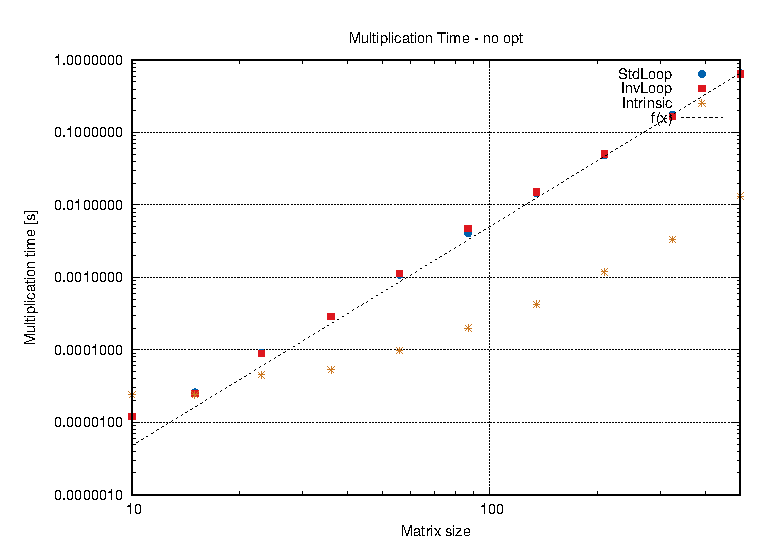
\includegraphics[width=.48\textwidth]{O0.eps}
\label{fig:no_optimization} }
\subfloat{    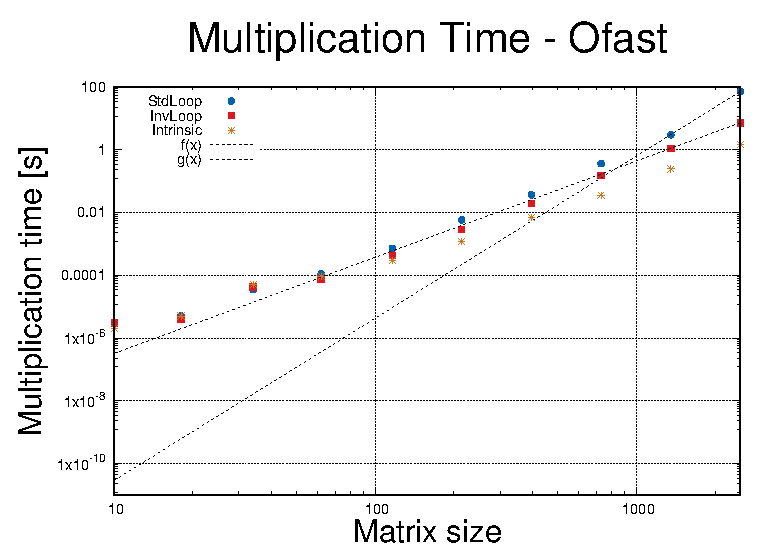
\includegraphics[width=.48\textwidth]{Ofast.eps}
\label{fig:Ofast}}
\caption{Computation time as a function of the matrix size, with or without optimization flags.}
\label{fig:timevsize}
\end{figure}
On graph I plotted power laws $f(x) = ax^b,$ with $a,b$ parameters retrieved from the data via fit; these power laws look like straight lines on these plots because of the double logarithmic scale.
The agreement between data and the power law is good for the "InvLoop" method (non-optimized), while is poor for the others; fit results for "Intrinsic" multiplication method are not shown since this data present an evident nonlinear behavior in both log-log plots.

\noindent These graphs suggest that the computation times scale as power laws with the matrix size, at least for user-implemented methods.
This statement might be verified building a more complex test involving repeated runs of the Python script, the elaboration of the data on a statistical base and the construction of confidence intervals.

Building this program I learned for the first time how to write a Python script and some ways to pass arguments between different languages.




\end{document}
